\documentclass[journal]{IEEEtai}

\usepackage{cite}
\usepackage{amsmath,amssymb,amsfonts}
\usepackage{mathtools}
\usepackage{bm}
\usepackage{booktabs}
\usepackage{multirow}
\usepackage{graphicx}
\usepackage{array}
\usepackage{xcolor}
\let\labelindent\relax
\usepackage{enumitem}
\usepackage[colorlinks,urlcolor=blue,linkcolor=blue,citecolor=blue]{hyperref}

\graphicspath{{../complement_paper/fig/}{../saseg_paper/}}

\newcommand{\known}{\textit{known}}
\newcommand{\unknown}{\textit{unknown}}
\newcommand{\cK}{\mathcal{K}}
\newcommand{\cUs}{\mathcal{U}_{\mathrm{seen}}}
\newcommand{\cUu}{\mathcal{U}_{\mathrm{unseen}}}
\newcommand{\Cand}{\mathcal{C}}
\newcommand{\CCG}{\textsc{CCG}}
\newcommand{\samthree}{SAM~3}
\newcommand{\samtwo}{SAM~2}
\DeclareMathOperator*{\argmax}{arg\,max}

\begin{document}

\title{From Unknown Detection to Structured Unknown Segmentation:\\Zero-Shot Candidate Generation for Open-World Dense Prediction}

\author{}

\markboth{IEEE Transactions on Artificial Intelligence, Vol. 00, No. 00, Month 202x}{From Unknown Detection to Structured Unknown Segmentation}

\maketitle

\begin{abstract}
Open-world dense segmentation requires more than assigning high anomaly scores to unfamiliar pixels: a usable system must also organize unknown evidence into spatially coherent regions while preserving predictions for known classes. We study this gap between \emph{unknown detection} and \emph{unknown structuring}. Across medical and natural-image segmentation settings, previously obtained diagnostic runs show that strong pixel-level ranking can coexist with nearly unusable unknown masks; for example, foreground AUROC exceeds 0.95 on four datasets while unknown F1 remains near zero. Region-level analysis further localizes the failure to candidate generation: the available representation can separate promising and unpromising proposals, yet the generated masks are poorly aligned with true unknown regions. Motivated by this diagnosis, we introduce \textbf{Complement Candidate Generation (\CCG)}, a zero-shot inference-time mechanism that uses concept-promptable segmentation to explain known content, extracts the residual foreground complement, decomposes that residual into mask candidates, and uses a frozen anomaly score only for region-level selection. Controlled interventions show that stronger scoring alone produces negligible improvement, whereas stronger candidates drive the dominant gain. Under the unified evaluation pipeline, unknown F1 on PASCAL VOC increases from 0.008 to 0.372 while known mIoU remains approximately 0.746; RoadAnomaly21 and RoadObstacle21 improve from 0.380 to 0.652 and from 0.054 to 0.515, respectively. Cityscapes shows a real but non-free gain, while medical CT forms a failure boundary because concept grounding is insufficient. The results support a narrower conclusion than architectural superiority: in the studied unseen-unknown settings, spatial candidate quality is the dominant missing capability between anomaly evidence and structured unknown output, and complement-based zero-shot candidates can bridge this gap when known-concept grounding is sufficiently complete.
\end{abstract}

\begin{IEEEImpStatement}
Open-world segmentation systems may recognize that a region is unfamiliar without producing an output that a downstream user can inspect, measure, or hand off. This work separates these two capabilities and shows that a high-quality anomaly score alone can be operationally insufficient. The proposed inference-time mechanism turns residual, unexplained foreground into explicit mask candidates and then uses anomaly evidence to select among them. This decomposition may help designers evaluate open-world systems at the level of usable regions rather than relying only on ranking metrics. The study also identifies clear limitations: dense scenes create known--unknown trade-offs, and out-of-domain modalities can invalidate the mechanism when known concepts cannot be grounded reliably. These boundaries should be considered before deployment in safety-critical workflows.
\end{IEEEImpStatement}

\begin{IEEEkeywords}
anomaly segmentation, open-world segmentation, structured abstention, zero-shot segmentation, foundation models, candidate generation
\end{IEEEkeywords}

\section{Introduction}
\label{sec:intro}

\IEEEPARstart{D}{ense} segmentation models are normally trained under a closed-set assumption: every pixel is expected to belong to one of the categories represented during training. In open-world deployment, that assumption fails. Images can contain novel objects, structures, pathologies, or scene elements that do not belong to the known label space. A conventional segmenter nevertheless assigns these pixels to the most similar known class, often with high confidence. Open-set recognition and out-of-distribution (OoD) detection address this failure by estimating whether an input or pixel is outside the known distribution~\cite{hendrycks2017baselinedetecting,liu2020energyout,yang2024generalizedout}. For dense prediction, however, identifying risk is only part of the problem.

A pixel-level risk map answers the question \emph{where is the model uncertain or unfamiliar?}. A structured unknown prediction must answer an additional question: \emph{which pixels belong together as an abstention region?} This distinction matters whenever the output is consumed spatially---for example, when an unfamiliar object must be handed to a human reviewer, when the size or extent of an unexplained region is measured, or when downstream logic operates on connected regions rather than independent pixels. Mask-level anomaly methods such as RbA and Mask2Anomaly already motivate region-based reasoning for unknown content~\cite{nayal2023rba,rai2024mask2anomaly}; our focus is complementary: we ask what prevents strong unknown evidence from becoming a usable structured output.

The empirical starting point of this paper is a repeated failure mode. Under an unseen-unknown setting, anomaly scores can achieve strong foreground AUROC while the resulting unknown F1 remains close to zero. This is not explained by a single architecture. A standard per-pixel $K{+}1$ model exhibits the same pattern: its direct unseen-unknown mask collapses while post-hoc MSP/Energy ranking remains strong. The important question is therefore not whether one query architecture outperforms a conventional $K{+}1$ segmenter, but why ranking information fails to become spatial structure.

We analyze the failure in two stages. First, region-level diagnostics show that the candidate masks available to the structured predictor are poorly aligned with the true unseen-unknown regions. Second, a proposal-conditioned analysis shows that the feature representation is already highly separable: matched and unmatched proposal tokens reach a linear-probe AUROC of 0.991, yet lightweight mask re-drawing remains far below the proposal upper bound. Together, these observations localize the dominant missing capability to \emph{candidate generation}: the system has useful evidence about unknownness but lacks spatially aligned masks on which that evidence can act.

This diagnosis suggests an intervention that does not require learning the semantics of every possible unknown class. Instead of asking a foundation model to ``segment the unknown,'' we ask it to explain the known part of the scene. A concept-promptable model enumerates masks for the known vocabulary; their union forms a partial explanation of the foreground; and the residual foreground complement becomes a source of unknown candidates. We call this mechanism \textbf{Complement Candidate Generation (\CCG)}. A frozen anomaly score is then aggregated over each candidate and used for region-level selection. The foundation-model branch is used only at inference time and requires no labels from the held-out unseen-unknown categories.

The central evidence is intervention-based. If score quality were the main bottleneck, replacing the score while holding candidates fixed should substantially improve structured unknown F1. It does not. On PASCAL VOC, a stronger-score intervention changes unknown F1 from approximately 0.008 to 0.007, whereas replacing the candidates while retaining the original score raises F1 to approximately 0.372. Cityscapes shows the same qualitative ordering in a more contaminated dense-scene regime. These results convert the original correlational diagnosis into a direct mechanism test.

The paper makes three contributions:
\begin{enumerate}[leftmargin=*]
    \item \textbf{Diagnosis.} We show that high anomaly-ranking quality can coexist with failed structured unknown output and localize the dominant bottleneck, in the studied unseen-unknown settings, to spatial candidate generation rather than score quality.
    \item \textbf{Method.} We introduce \CCG, a zero-shot inference-time mechanism that constructs unknown candidates by explaining known content, taking its foreground complement, and using a frozen anomaly score for region-level selection.
    \item \textbf{Boundary characterization.} Using existing experiments across natural images, road-scene anomaly benchmarks, and medical CT, we characterize effective, trade-off, and failure regimes and relate them to known-concept grounding coverage and candidate contamination.
\end{enumerate}

Importantly, we do \emph{not} claim that native unknown queries are necessary, that a particular structured-abstention architecture is universally superior to $K{+}1$ segmentation, or that the proposed mechanism solves unseen-unknown structuring in every domain. The evidence supports a narrower and more reusable conclusion: strong evidence needs spatially usable candidates, and the quality of those candidates governs whether unknown detection can become structured prediction.

\section{Related Work}
\label{sec:related}

\subsection{Open-Set Recognition and Dense OoD Detection}
Open-set recognition and OoD detection estimate whether samples fall outside a known training distribution~\cite{hendrycks2017baselinedetecting,liu2020energyout,bendale2016towardsopen,zhou2021learningplaceholders,yang2024generalizedout}. Dense variants transfer this idea to pixels, often using confidence, energy, uncertainty, or outlier exposure. These methods are essential because they provide the anomaly evidence used by our selection stage. Their ranking metrics, however, do not by themselves specify how anomalous pixels should be assembled into a coherent region. Our experiments explicitly separate ranking quality from the spatial candidate set on which a structured predictor operates.

\subsection{Mask-Based Unknown and Anomaly Segmentation}
Mask-based segmentation established region-level prediction as an alternative to independent per-pixel classification. MaskFormer, Mask2Former, and Mask DINO provide canonical query/mask formulations~\cite{cheng2021perpixel,cheng2022mask2former,li2022maskdino}. RbA uses mask-classification queries as one-vs-all classifiers and scores unknown regions by rejection from known classes~\cite{nayal2023rba}. Mask2Anomaly further develops mask-level open-set segmentation with global masked attention, contrastive learning, unknown mining, and mask refinement~\cite{rai2024mask2anomaly}. These works establish that mask-level reasoning is relevant to unknown segmentation. Our contribution is not a claim that mask classification itself is new; rather, we isolate the candidate-generation bottleneck under unseen-unknown transfer and intervene on candidate structure without retraining the primary segmentation model.

\subsection{Promptable and Open-Vocabulary Foundation Models}
Foundation models for segmentation have progressively expanded the prompt interface from points and boxes to concept-level grounding. SAM~2 provides promptable segmentation for images and video~\cite{ravi2024sam2}, while SAM~3 introduces promptable concept segmentation, accepting open-vocabulary text or exemplar concepts and returning matching masks~\cite{carion2025sam3}. CLIP provides a complementary language--vision representation that supports zero-shot concept transfer~\cite{radford2021clip}. We use concept promptability in a deliberately asymmetric way: the model is not asked to name unknown content. It is asked to explain known concepts; unexplained foreground becomes the candidate source.

\subsection{Anomaly Segmentation Benchmarks}
SegmentMeIfYouCan (SMIYC) provides real-world anomaly and obstacle segmentation tracks for road scenes~\cite{chan2021smiyc}. These benchmarks are useful external checks because they contain both pixel- and instance-oriented evaluation. We use RoadAnomaly21 and RoadObstacle21 as cross-benchmark mechanism validation, not as evidence of leaderboard superiority: the proposed method is attached to a Cityscapes-trained checkpoint without task-specific retraining.

\section{Problem Formulation: From Evidence to Structure}
\label{sec:problem}

\subsection{Label Regimes}
Let $\cK$ denote the known classes, $\cUs$ categories available as a generic unknown class during development, and $\cUu$ categories held out as unknown until evaluation. We use two regimes only as experimental controls:
\begin{itemize}[leftmargin=*]
    \item \textbf{Seen-unknown control (A1).} Pixels from $\cUs$ are supervised as a generic unknown class and evaluated on the same seen-unknown category set. This is best viewed as supervised $K{+}1$ segmentation, not as unseen-category discovery.
    \item \textbf{Unseen-unknown structuring (A2).} The model may have generic unknown supervision from $\cUs$, but no labels from $\cUu$ are used in training. Evaluation asks whether held-out unknown categories can be represented as structured unknown regions.
\end{itemize}
This positioning is intentionally conservative. A1 is useful for showing that explicit unknown output can be learned under supervision; the main scientific question of this paper is A2.

\subsection{Evidence, Candidates, and Structured Output}
For an image $I$, let $s(x)$ be a pixel-level anomaly score. Ranking metrics such as AUROC and AUPR evaluate whether $s(x)$ orders unknown pixels above known pixels, but do not encode objectness or region membership.

Let $\Cand=\{C_i\}_{i=1}^{N}$ be a set of spatial candidates. A region-level selector aggregates anomaly evidence over each candidate,
\begin{equation}
  S(C_i)=\frac{1}{|C_i|}\sum_{x\in C_i}s(x),
\end{equation}
and produces the structured unknown output
\begin{equation}
  \hat{U}=\bigcup_{i:S(C_i)>\tau} C_i.
\end{equation}
This decomposition makes the failure modes explicit. A system can fail because $s(x)$ is weak, because $\Cand$ has low coverage or purity, or because the region selector is poorly calibrated. Our experiments are organized around interventions that distinguish these possibilities.

\subsection{Metrics}
We report Known mIoU for known-class segmentation; Unknown F1, IoU, precision, and recall for the final structured output; and AUROC/AUPR/FPR@95 for pixel-level ranking when available. Candidate diagnostics include union IoU, candidate precision, candidate recall, and hit rate at a minimum candidate/ground-truth IoU. We avoid interpreting a high AUROC as evidence of successful structured segmentation.

\section{Diagnosing the Detection--Structuring Gap}
\label{sec:diagnosis}

\subsection{A1 as a Supervised Control}
The seen-unknown setting clarifies what should and should not be claimed. On Synapse, a standard independently trained per-pixel $K{+}1$ segmenter reaches Unknown F1 $0.797$, compared with $0.721$ for the structured query-based baseline. Thus the data do not establish superiority of native unknown queries. Instead, they show that reserving an explicit unknown output is sufficient to learn structured rejection when the unknown categories are supervised.

\begin{table}[t]
\centering
\caption{Synapse seen-unknown control (single seed for independent architectures). A1 is treated as supervised $K{+}1$ segmentation rather than a claim of open-world discovery.}
\label{tab:a1_control}
\footnotesize
\begin{tabular}{lccc}
\toprule
Method & Known mIoU & Unknown F1 & Unknown IoU \\
\midrule
PerPixel-$K$ + Energy (post-hoc) & 0.829 & 0.024 & --- \\
PerPixel-$K{+}1$ (direct) & 0.825 & \textbf{0.797} & \textbf{0.663} \\
Structured query baseline & 0.811 & 0.721 & 0.564 \\
\bottomrule
\end{tabular}
\end{table}

\subsection{High Ranking Quality, Near-Zero Structured F1}
The main A2 diagnostic runs show a consistent gap between ranking and structuring. Table~\ref{tab:gap} reports the original diagnostic pipeline results. The absolute values are not reused as the baseline for the later complement-method comparison; they serve only to establish the failure mode under the diagnostic setup.

\begin{table}[t]
\centering
\caption{Detection--structuring gap in the original A2 diagnostic runs. Strong foreground ranking coexists with near-zero structured unknown F1.}
\label{tab:gap}
\footnotesize
\begin{tabular}{lccc}
\toprule
Dataset & AUROC$_{\rm fg}$ & AUPR$_{\rm fg}$ & Unknown F1 \\
\midrule
Synapse & 0.971 & 0.088 & 0.006 \\
AMOS22 & 0.990 & --- & 0.010 \\
PASCAL VOC & 0.970 & 0.671 & 0.002 \\
Cityscapes & 0.956 & 0.208 & 0.022 \\
\bottomrule
\end{tabular}
\end{table}

This pattern is also visible in an independently trained per-pixel $K{+}1$ A2 baseline on Synapse: its direct unseen-unknown output collapses to F1 $0.004$, while post-hoc MSP reaches AUROC $0.981$. The gap is therefore not specific to a query parser.

\subsection{Candidate Alignment Is the Missing Step}
Region-level analysis localizes the failure more precisely. The baseline unknown-slot candidates have union IoU $0.005$ with held-out unknown regions and a slice hit rate of only $0.02$ at IoU$\geq0.10$. In contrast, connected components extracted from the top $0.3\%$ of the ensemble anomaly map reach union IoU $0.153$ and hit rate $0.70$. This indicates that useful localization evidence exists but is not being converted into suitable masks.

A linear separability test further rules out the absence of discriminative representation as the main explanation. Proposal tokens corresponding to matched and unmatched candidates reach linear-probe AUROC $0.991$ with centroid distance $8.95$. Yet direct mask re-drawing from those tokens remains weak, and residual local refinement improves but does not close the gap to the proposal upper bound. The remaining problem is therefore structural: how to generate coherent masks that align with unseen unknown regions.

\begin{table}[t]
\centering
\caption{Existing proposal/refinement diagnostics on Synapse A2.}
\label{tab:proposal_diag}
\footnotesize
\begin{tabular}{lccc}
\toprule
Variant & Union IoU & Hit@0.10 & Comp. Prec.@0.10 \\
\midrule
Baseline unknown-slot candidates & 0.005 & 0.020 & --- \\
Direct re-drawing & 0.039 & 0.080 & 0.048 \\
Residual refinement & 0.071 & 0.420 & 0.169 \\
Best lightweight refinement & 0.073 & 0.440 & 0.172 \\
Ensemble-proposal upper bound & \textbf{0.153} & \textbf{0.700} & \textbf{0.188} \\
\bottomrule
\end{tabular}
\end{table}

These diagnostics motivate a direct candidate intervention rather than further score sharpening.

\section{Complement Candidate Generation}
\label{sec:method}

\subsection{Overview}
\CCG is an inference-time candidate generator attached to a frozen open-world segmentation system. The base system supplies (i) known-class predictions and (ii) a pixel-level anomaly score. The foundation-model branch supplies spatial structure. The pipeline has four stages: known-concept enumeration, known-union construction, foreground complement extraction and decomposition, and region-level score fusion.

The method does not require labels from $\cUu$, does not fine-tune the concept-promptable foundation model, and does not retrain the base segmentation checkpoint. It does, however, inherit whatever generic seen-unknown supervision was used to train the frozen A2 checkpoint; we therefore describe the method as zero-shot with respect to the held-out unseen categories, not as supervision-free open-world learning.

\subsection{Known-Concept Enumeration}
Let $\mathcal{V}_{K}=\{c_1,\ldots,c_K\}$ be the vocabulary of known semantic classes. For each concept $c_k$, a concept-promptable model returns one or more masks $M_k$. Their union forms a known explanation of the scene,
\begin{equation}
  M_{\mathrm{known}} = \bigcup_{k=1}^{K} M_k.
\end{equation}
The purpose is not to replace the task segmenter. The union only estimates which foreground regions can already be explained by known concepts.

\subsection{Foreground Complement and Candidate Decomposition}
Let $M_{\mathrm{fg}}$ denote the foreground support used by the pipeline. The residual is
\begin{equation}
  M_{\mathrm{comp}} = M_{\mathrm{fg}} \setminus M_{\mathrm{known}}.
\end{equation}
A class-agnostic mask generator decomposes $M_{\mathrm{comp}}$ into candidate masks $\Cand=\{C_i\}$. Lightweight geometric filtering removes tiny regions and candidates heavily overlapping the known union:
\begin{align}
  \mathrm{area}(C_i) &> \tau_{\mathrm{area}},\\
  \mathrm{overlap}(C_i,M_{\mathrm{known}}) &< \tau_{\mathrm{overlap}}.
\end{align}
This ``explain known, then inspect the residual'' strategy is intentionally different from prompting the model with words such as ``unknown'' or ``anomaly.'' Existing prompt-form ablations show that direct negation and negative-exemplar variants fail to produce useful masks, whereas enumeration-then-complement is consistently usable.

\subsection{Region-Level Anomaly Selection}
The residual is high recall but can contain known leakage. We therefore aggregate the frozen baseline score over each candidate. In the existing implementation,
\begin{equation}
 s_i = \frac{1}{|C_i|}\sum_{x\in C_i}\left[0.8\,(1-p_{\mathrm{best}}(x))+0.2\,U_{\mathrm{union}}(x)\right],
 \label{eq:score}
\end{equation}
where $p_{\mathrm{best}}$ is the best known-class confidence and $U_{\mathrm{union}}$ is the auxiliary unknown response from the frozen structured-abstention checkpoint. The final output is
\begin{equation}
 \hat{U}=\bigcup_{i:s_i>\tau_{\mathrm{fusion}}} C_i.
\end{equation}
We call the unfiltered candidate output \textbf{L1} and the full candidate-plus-score pipeline \textbf{L2}. L1 isolates candidate generation; L2 tests whether existing anomaly evidence can purify those candidates.

\subsection{Why the Decomposition Is Testable}
The method yields a falsifiable prediction. If score quality is the principal bottleneck, a stronger score with fixed candidates should improve structured F1 substantially. If candidate quality is the bottleneck, replacing candidates while retaining the original score should produce the dominant gain. Section~\ref{sec:intervention} tests exactly these interventions.

\section{Experiments}
\label{sec:experiments}

\subsection{Datasets and Roles}
The experiments use six datasets with different narrative roles. Synapse and AMOS22 provide medical diagnostic and failure-boundary evidence. PASCAL VOC 2012 is the primary positive natural-image setting. Cityscapes is a dense-scene trade-off case. RoadAnomaly21 and RoadObstacle21 test transfer under the SMIYC road-anomaly setting~\cite{chan2021smiyc}. The Cityscapes A2 checkpoint is reused for both road datasets without task-specific retraining.

The class partitions are fixed by the existing runs. Synapse uses eight known classes, three seen unknowns, and two unseen unknowns. AMOS22 uses eight known, four seen unknown, and three unseen unknown classes. VOC uses fifteen known, three seen unknown, and two unseen unknown classes. Cityscapes uses fourteen known, three seen unknown, and two unseen unknown classes. Exact category lists are provided in the supplementary material.

\subsection{Scope of the Existing Evidence}
This rewrite intentionally introduces no new model training or evaluation runs. We therefore distinguish two types of evidence. First, the diagnosis tables reproduce previously completed runs and are used to establish mechanisms rather than benchmark superiority. Second, the complement-method tables use the internally consistent evaluation pipeline from the candidate-generation study so that baseline and intervention variants are compared under the same code path. Where experiments use public validation data and validation-selected thresholds, we interpret the numbers as controlled mechanism evidence rather than as hidden-test generalization estimates. No claim of leaderboard state of the art is made.

\subsection{Main Full-System Results}
Table~\ref{tab:main_results} reports the unified A2 pipeline used by the complement study. On VOC, L1 demonstrates the expected high-recall/low-purity behavior: Unknown Recall reaches $0.994$, but Known mIoU drops sharply. L2 uses the frozen anomaly score to recover known-side quality while retaining most unknown recall, raising Unknown F1 from $0.008$ to $0.372$ with essentially unchanged Known mIoU. Cityscapes improves less cleanly: Unknown F1 rises from $0.017$ to $0.074$, while Known mIoU decreases from $0.624$ to $0.583$. The mechanism therefore works, but not for free, in dense urban scenes.

\begin{table*}[t]
\centering
\caption{Full-system A2 results from the unified candidate-generation evaluation pipeline. Road-scene rows reuse the Cityscapes checkpoint and report the same unknown-output metrics used in the mechanism study.}
\label{tab:main_results}
\footnotesize
\begin{tabular}{llcccccc}
\toprule
Dataset & Method & Known mIoU & Unknown F1 & Unknown IoU & Precision & Recall & AUROC$_{\rm fg}$ \\
\midrule
VOC & Baseline & 0.746 & 0.008 & 0.004 & 0.005 & 0.012 & 0.980 \\
VOC & L1 candidates & 0.334 & 0.175 & 0.096 & 0.096 & 0.994 & 0.731 \\
VOC & L2 (\CCG) & \textbf{0.746} & \textbf{0.372} & \textbf{0.228} & \textbf{0.231} & 0.954 & 0.981 \\
\midrule
Cityscapes & Baseline & 0.624 & 0.017 & 0.008 & 0.011 & 0.032 & 0.963 \\
Cityscapes & L1 candidates & 0.279 & 0.035 & 0.018 & 0.018 & 0.987 & 0.781 \\
Cityscapes & L2 (\CCG) & 0.583 & \textbf{0.074} & \textbf{0.038} & \textbf{0.047} & 0.140 & 0.962 \\
\midrule
RoadAnomaly21 & Baseline & --- & 0.380 & 0.234 & 0.433 & 0.338 & 0.828 \\
RoadAnomaly21 & L2 (\CCG) & --- & \textbf{0.652} & \textbf{0.484} & 0.506 & \textbf{0.916} & 0.885 \\
RoadObstacle21 & Baseline & --- & 0.054 & 0.028 & 0.037 & 0.103 & 0.949 \\
RoadObstacle21 & L2 (\CCG) & --- & \textbf{0.515} & \textbf{0.347} & 0.423 & \textbf{0.659} & 0.960 \\
\bottomrule
\end{tabular}
\end{table*}

\begin{figure}[t]
  \centering
  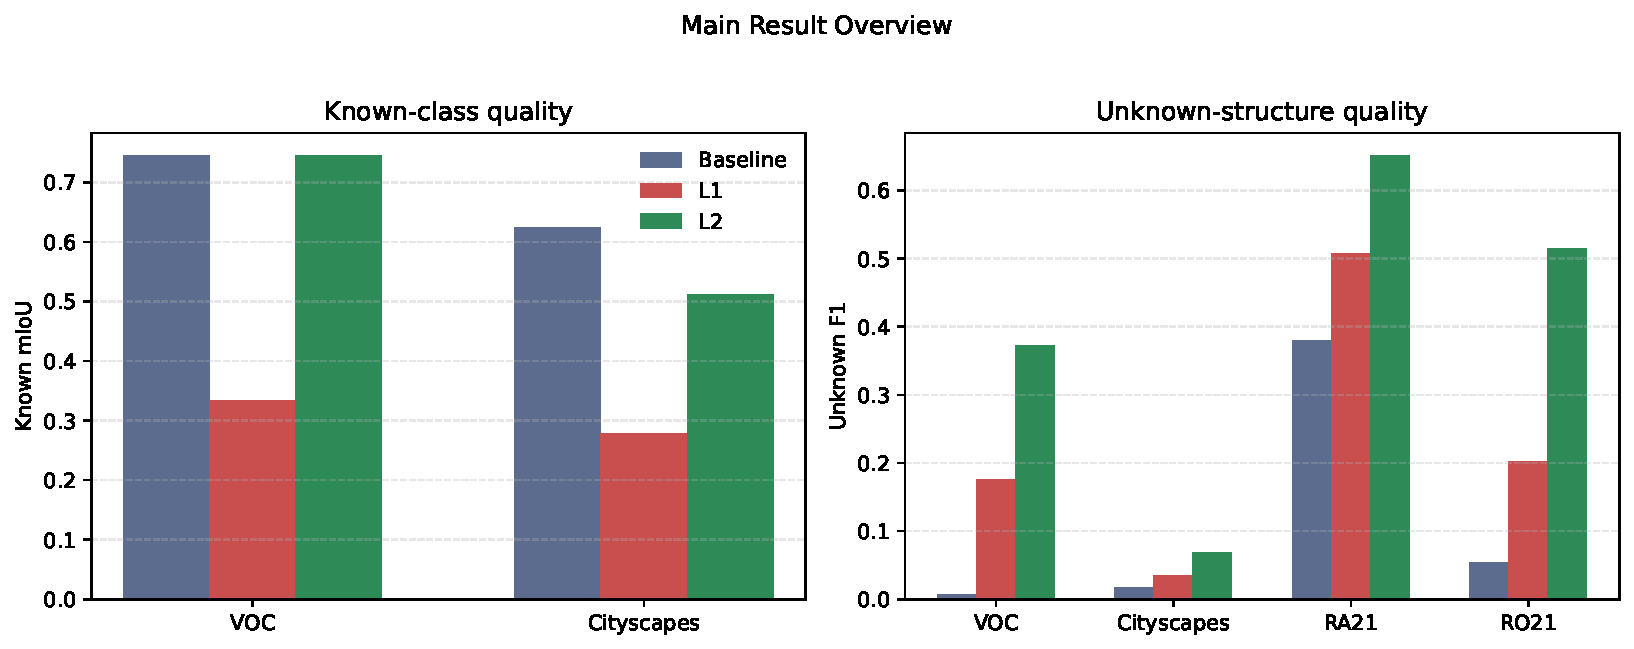
\includegraphics[width=\linewidth]{main_results_overview.pdf}
  \caption{Existing overview of full-system results. The central pattern is not uniform superiority but a strong positive regime on VOC, a trade-off regime on Cityscapes, and transfer gains on the road-scene datasets.}
  \label{fig:main_results}
\end{figure}

\subsection{Controlled Intervention: Score or Candidates?}
\label{sec:intervention}
The intervention experiment is the main causal-style mechanism test. We compare (A) a stronger score with the original candidates, (B) stronger complement-derived candidates with the original score, and (A+B) both changes together.

\begin{table}[t]
\centering
\caption{Controlled intervention. Candidate replacement drives the dominant structured-F1 gain.}
\label{tab:intervention}
\footnotesize
\begin{tabular}{llcc}
\toprule
Dataset & Setting & Known mIoU & Unknown F1 \\
\midrule
\multirow{4}{*}{VOC}
& Baseline & 0.746 & 0.008 \\
& A: stronger score only & 0.745 & 0.007 \\
& B: stronger candidates only & 0.746 & 0.372 \\
& A+B & 0.745 & 0.377 \\
\midrule
\multirow{4}{*}{Cityscapes}
& Baseline & 0.624 & 0.017 \\
& A: stronger score only & 0.624 & 0.015 \\
& B: stronger candidates only & 0.512 & 0.069 \\
& A+B & 0.497 & 0.064 \\
\bottomrule
\end{tabular}
\end{table}

On VOC, score replacement alone does not improve structured F1, whereas candidate replacement raises it by roughly two orders of magnitude. Adding the stronger score on top yields only a small additional gain. Cityscapes has noisier candidates, but the ordering remains: candidate replacement helps, while score sharpening alone does not. These results support the diagnosis that candidate generation, rather than ranking quality, is the dominant bottleneck in these A2 runs.

\begin{figure}[t]
  \centering
  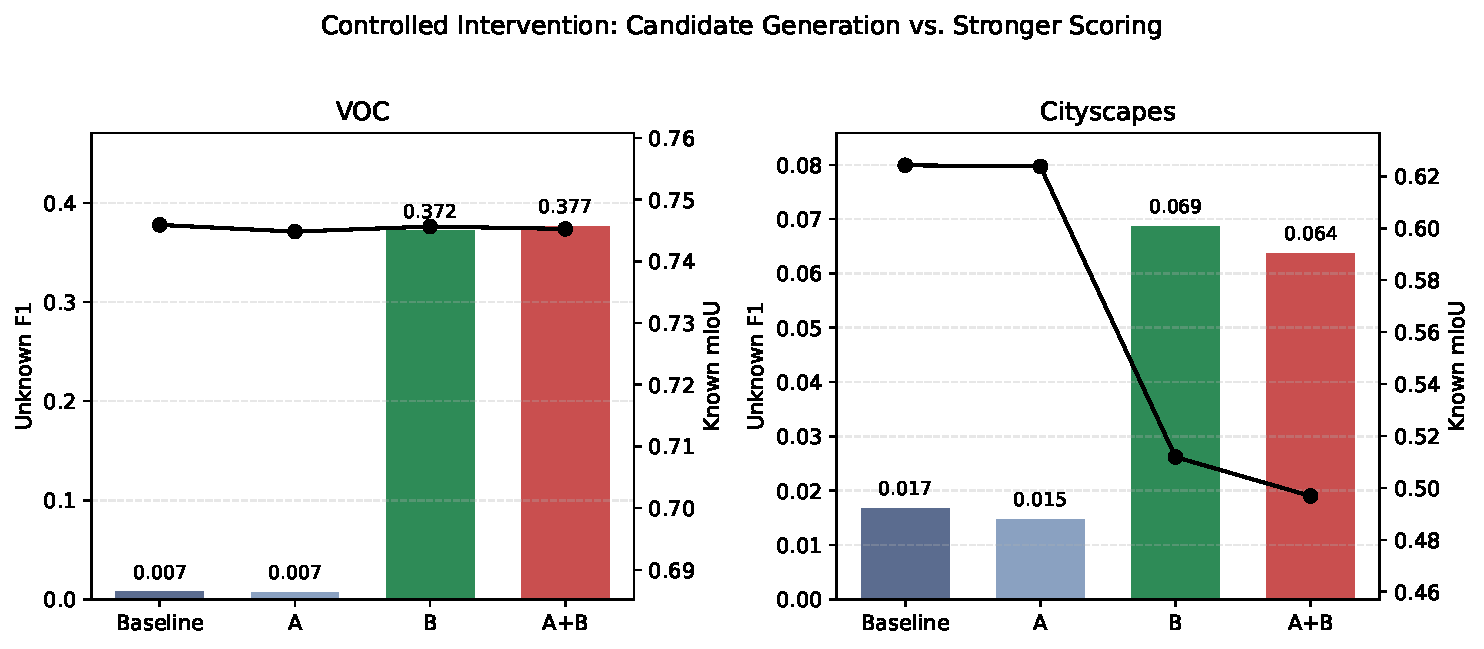
\includegraphics[width=\linewidth]{intervention_bar.pdf}
  \caption{Existing intervention visualization. Stronger candidates, not stronger scores, account for the main improvement.}
  \label{fig:intervention}
\end{figure}

\subsection{Why Complement Candidates Work or Fail}
Table~\ref{tab:candidate_quality} summarizes existing candidate diagnostics. VOC is the effective regime: the known union explains much of the known content, the complement retains nearly all unknown pixels, and precision remains high. Cityscapes is a contamination regime: unknown recall remains high, but known leakage is substantial. Synapse CT is a grounding-failure regime: only a subset of organ concepts are grounded reliably, so the residual cannot serve as a clean unknown proposal source.

\begin{table}[t]
\centering
\caption{Existing candidate-quality diagnostics before final score fusion.}
\label{tab:candidate_quality}
\footnotesize
\begin{tabular}{lcccc}
\toprule
Dataset & Known-union IoU & Comp. IoU & Unk. recall & Comp. precision \\
\midrule
VOC & 0.696 & 0.889 & 1.000 & 0.889 \\
Cityscapes & 0.532 & 0.171 & 0.990 & 0.171 \\
Synapse CT & 0.652 & --- & 0.936 & 0.045 \\
\bottomrule
\end{tabular}
\end{table}

The CT failure is especially informative. The complement has high recall because incomplete known grounding leaves large residual areas, but precision is only $0.045$ and known leakage is approximately $0.955$. This is not a score-selection problem; the candidate source itself is invalid because the known explanation is incomplete.

\begin{figure}[t]
  \centering
  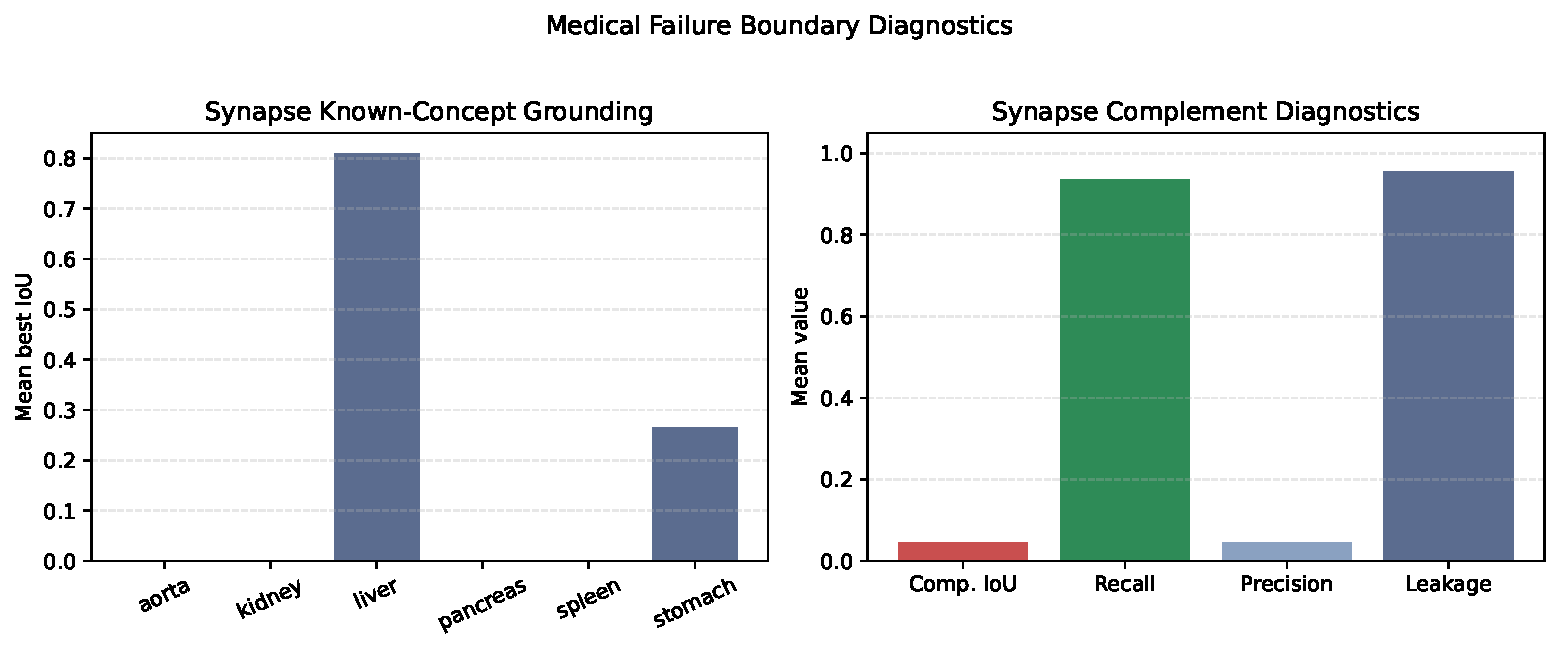
\includegraphics[width=\linewidth]{medical_diagnostics.pdf}
  \caption{Existing medical failure diagnostics. Weak concept grounding makes the complement dominated by known anatomy rather than meaningful unknown candidates.}
  \label{fig:medical}
\end{figure}

\subsection{Prompt Form and Backbone Dependence}
Direct negation is not a reliable route to unknown discovery with the current concept-promptable interface. On the existing diagnostic subsets, direct negation yields zero unknown-mask recall; generic concepts and negative exemplars are weak; enumeration-then-complement is the only prompt form that consistently produces useful candidates. This supports interpreting \CCG as a residual-explanation mechanism rather than a generic prompt-engineering recipe.

A backbone substitution provides a second check. On VOC, native \samthree{} concept segmentation with L2 reaches Unknown F1 $0.372$, whereas an orchestrated \samtwo{}+CLIP alternative reaches $0.222$ while maintaining Known mIoU $0.739$. On Cityscapes the alternative reaches F1 $0.033$ versus $0.074$ for native \samthree{}. The effect is therefore not exclusive to a single model instance, but it depends on the joint quality of concept grounding and class-agnostic mask generation.

\begin{table}[t]
\centering
\caption{Backbone substitution under the existing full-system A2 setting.}
\label{tab:backbone}
\footnotesize
\begin{tabular}{lcc}
\toprule
Backbone & VOC mIoU / F1 & Cityscapes mIoU / F1 \\
\midrule
Baseline & 0.7459 / 0.0075 & 0.6242 / 0.0167 \\
\samthree{} + L2 & 0.7457 / 0.3719 & 0.5833 / 0.0736 \\
\samtwo{}+CLIP + L2 & 0.7393 / 0.2224 & 0.6222 / 0.0330 \\
\bottomrule
\end{tabular}
\end{table}

\subsection{Qualitative Regimes}
Figure~\ref{fig:qualitative} summarizes the three regimes using existing visualizations. VOC shows a clean complement and successful purification. Cityscapes shows unknown recovery together with known leakage in dense scenes. Medical CT shows failure at the concept-grounding stage. These examples make the distinction between anomaly evidence and candidate structure visible: a strong score cannot recover an object mask that was never proposed correctly.

\begin{figure*}[t]
  \centering
  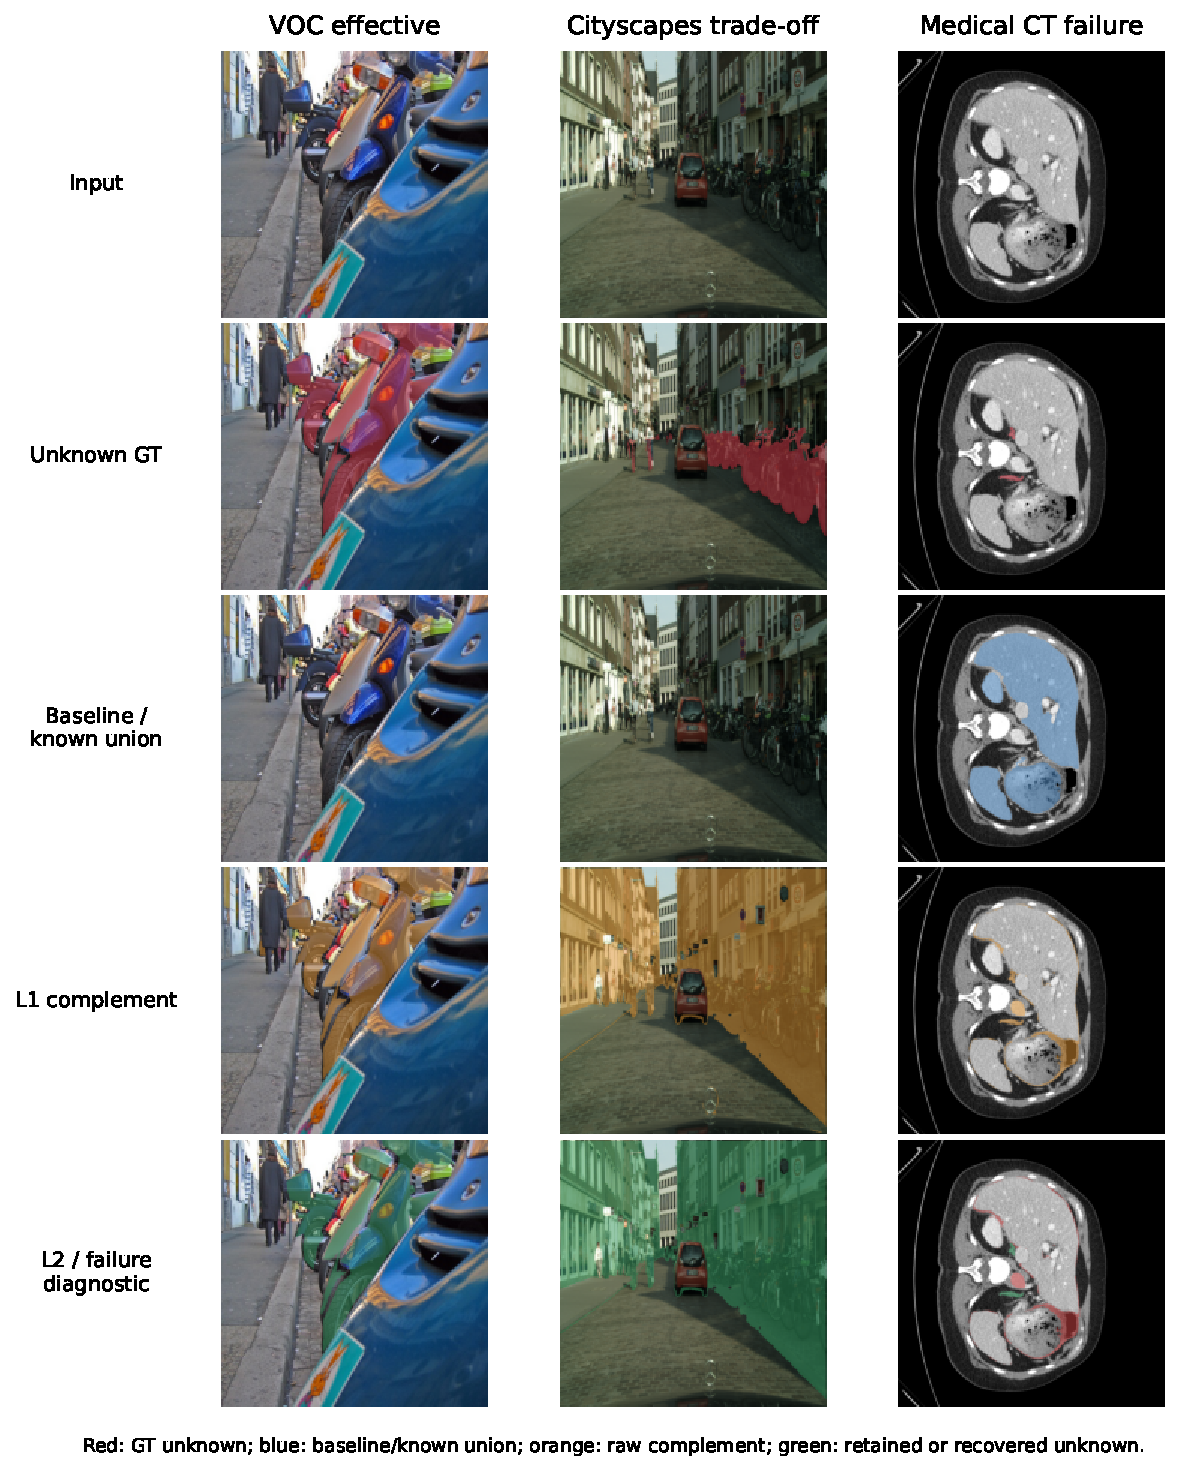
\includegraphics[width=0.95\textwidth]{qualitative_triptych.pdf}
  \caption{Existing qualitative examples for the effective (VOC), trade-off (Cityscapes), and failure (medical CT) regimes.}
  \label{fig:qualitative}
\end{figure*}

\subsection{Road-Scene External Evaluation}
The SMIYC public-validation evaluator reveals an additional limitation. L2 improves the pixel-level AP/Best-F1 metrics on both RoadAnomaly21 and RoadObstacle21, but L1 can be substantially stronger on instance-oriented SegEval F1. Mean-score mask filtering improves pixel purity while sometimes discarding or fragmenting large anomalies with spatially non-uniform scores. This divergence is useful because it shows that candidate generation and candidate selection should be evaluated at both pixel and instance levels; the current L2 selector is not instance preserving.

\section{Discussion}
\label{sec:discussion}

\subsection{What the Results Do and Do Not Establish}
The results support a decomposition rather than an architecture ranking. The seen-unknown control shows that a conventional $K{+}1$ output can perform strongly when unknown categories are supervised. The unseen-unknown diagnostics show that both query-based and per-pixel models can retain strong anomaly ranking while their direct structured outputs fail. The intervention results then show that changing the candidate set has a much larger effect than changing the score. Taken together, the evidence supports candidate generation as the dominant missing capability in the studied A2 runs.

This conclusion is deliberately narrower than saying that scoring never matters. L1 demonstrates the opposite: high-recall candidates can destroy known-class quality if they are accepted without selection. The division of labor is therefore: candidate generation supplies spatial structure; scoring supplies selectivity. The bottleneck diagnosis concerns which component is missing when ranking is already strong but structured F1 is near zero.

\subsection{Why Complementation Is Conditional}
\CCG assumes that the known vocabulary can be grounded with enough coverage that the residual foreground is meaningful. When this assumption holds, as in the VOC diagnostic subset, the complement is both high recall and reasonably pure. When grounding is partial in dense scenes, the complement is contaminated by known residue and score fusion faces a difficult known--unknown trade-off. When grounding collapses out of domain, as in the CT experiments, the complement ceases to represent ``unexplained unknown'' and becomes mostly ``unexplained known.'' The foundation model is therefore a candidate generator, not a universal unknown recognizer.

\subsection{Relation to Structured Abstention}
The term \emph{structured abstention} is useful as an output-level requirement: instead of returning only a scalar or pixel-wise alarm, the system reserves an explicit spatial region for content it cannot explain safely. The present paper does not require a specific decoder architecture to realize that requirement. A supervised $K{+}1$ class, a mask-classification query, or a candidate-selection pipeline can all instantiate structured abstention under different regimes. The contribution here is to identify the extra candidate-generation capability required when the unknown category itself is held out.

\subsection{Limitations}
First, the current evidence reuses existing experimental runs. Some public-validation results use validation-selected operating points; we therefore treat them as controlled mechanism studies rather than unbiased hidden-test estimates. A future submission aimed at benchmark ranking should repeat the load-bearing comparisons on a fully held-out test protocol.

Second, the dense-scene trade-off remains unresolved. Cityscapes improves unknown F1 only with a measurable known-mIoU cost. Third, the current foundation model has insufficient medical concept grounding, so the zero-shot complement mechanism is not directly applicable to CT. Fourth, mean-score candidate filtering is not instance preserving, as shown by SMIYC SegEval. Fifth, the intervention evidence is strongest on VOC and Cityscapes; the broader cross-dataset conclusions should be read as qualitative boundary characterization rather than universal statistical claims.

\section{Conclusion}
We studied why strong unknown-detection evidence can fail to produce structured unknown regions in open-world dense segmentation. Existing diagnostic runs show that high AUROC can coexist with near-zero unknown F1 and that useful representation-level separation does not guarantee spatially aligned masks. This localizes the missing capability to candidate generation. We then introduced Complement Candidate Generation, which explains known content with a concept-promptable model, decomposes the residual foreground into candidate masks, and uses a frozen anomaly score for region-level selection. Controlled interventions show that candidate replacement drives the main structured-F1 gain, whereas score strengthening alone is ineffective in the studied A2 settings. The mechanism succeeds when known-concept grounding is sufficiently complete, trades off in dense scenes with substantial leakage, and fails when grounding collapses out of domain. These findings suggest that open-world dense prediction should evaluate not only whether a model can rank unfamiliar pixels, but also whether it can generate spatial candidates that make abstention operationally usable.

\bibliographystyle{IEEEtran}
\bibliography{../saseg_paper/references,references_additions}

\end{document}
